%
% FH Technikum Wien
% !TEX encoding = UTF-8 Unicode
% LTeX: language=en
%
% Preparing master's and bachelor's theses at UAS Technikum Wien using LaTeX and the TWBOOK class
%
% To create your own document, complete the following steps:
% 1) Configure \documentclass[..]
%    * Master's or bachelor's thesis
%      * Master   ... master's thesis
%      * Bachelor ... bachelor's thesis
%    * Language (english, german, ngerman)
%    * Citation standard (Harvard, IEEE) (default: IEEE)
%    * Biber or BibTeX as the bibliography backend (Biber, BibTeX) (default: Biber)
% 2) Enter the degree course
% 3) Complete the title page, abstract, etc.
% 4) Write the thesis (enter the literature sources used in Literatur.bib)
%
% Tested with TeXstudio using UTF-8 character encoding (= ansinew/latin1) and TeX Live on Ubuntu
% Note that the file encoding must match the encoding specified for the inputenc package!
% The encoding of the twbook.cls file MUST be ANSI!
% When using UTF-8, both the document and the BibTeX file must be encoded as UTF-8!
%
% Please send bug reports and feedback by email to latex@technikum-wien.at
%
% Version V2.24 from 2024-12-19, otrebski
%
\documentclass[Master,english,IEEE]{twbook}
\usepackage[utf8]{inputenc}
\usepackage[T1]{fontenc}
\usepackage{todonotes}
\usepackage{booktabs}
\usepackage{tabularx}
\usepackage{amsmath}
\usepackage{tikz}
\usetikzlibrary{positioning,calc,arrows.meta}

\newcommand{\R}{$\text{R}^2$} 
% Enter the degree course here
\degreecourse{Data Science}

\addbibresource{Literatur.bib}
\addbibresource{master-thesis.bib}

%% Define additional bibliography databases here if required

% The following packages provide otherwise unavailable features
\usepackage{blindtext}

%
% Entries for the title page, abstract, etc.
%
\title{Title of the Thesis\todo[inline]{replace}}
\author{David Zelenay, BSc.}
\studentnumber{XXXXXXXXXXXXXXX \todo[inline]{replace}}
%\author{Title First Name Last Name, Degree\and{}Title First Name Last Name, Degree}
%\studentnumber{XXXXXXXXXXXXXXX\and{}XXXXXXXXXXXXXXX}
\supervisor{FH-Prof. Priv.-Doz. Mag. Dr. David Meyer}
%\supervisor[Reviewer]{Title First Name Last Name, Degree}
%\supervisor[Reviewer]{Title First Name Last Name, Degree}
%\secondsupervisor{Title First Name Last Name, Degree}
%\secondsupervisor[Reviewer]{Title First Name Last Name, Degree}
%\secondsupervisor[Reviewers]{Title First Name Last Name, Degree}
\place{Vienna}
\kurzfassung{\blindtext\todo[inline]{replace}}
\schlagworte{Keyword1, Keyword2, Keyword3, Keyword4 \todo[inline]{replace}}
\outline{\blindtext\todo[inline]{replace}}
\keywords{Keyword1, Keyword2, Keyword3, Keyword4\todo[inline]{replace}}
%\acknowledgements{\blindtext}

\begin{document}

\maketitle
% TODO Add math mode to all columns containing decimal numbers in tables.
% TODO Format whole document
% TODO check where Table 10 is.
\chapter{Introduction}

\section{Motivation}

\section{Research Questions}

\begin{enumerate}
    \item Which forecast approach performs best for the given data?
    \item How do neighboring stations and weather data affect the forecast performance?
    \item How does the forecast performance change with lead time?
    \item In which scenarios does the model excel and in which does it struggle?
\end{enumerate}
\chapter{Methodology}
% ~ 20%
% The second chapter should explain the methods used for answering the research questions. This includes the process as well as all empirical and technical tools. The description will naturally be based on literature, in the sense that it will refer to it – but note that it must not be a summary of basics (such as: “What is a neural network?”) but precisely explain how the methods are used (for example: what kind of network architecture is used for this work, how it is trained, how the hyperparameters are tuned etc.) and why (what are the alternatives?). The description must be detailed enough to allow the reproduction of the results. Assume that the reader is familiar with everything taught in the courses of the data science study program. Standard methods should not be described at all, specialized methods only shortly, and references given.


\section{Water Level Data}
The main data source for the thesis is the FloodAlert water level data \cite{FloodAlertWaterLevels}. To limit the scope of the thesis a single station is selected as the forecasting target. The target station is on the Danube and located in Korneuburg (a suburb of Vienna). The main reasons for selecting this station are the availability and quality of the data, as well as its popularity 
(measured by notification subscribers). % TODO Check with Johannes if I can include that
Additionally the station has multiple upstream measurement stations, which allows for the investigation of the effect of upstream data on forecast performance. 

Each station provides at most two features: water level and flow rate. Since not every station provides both features, the flow rate has been dismissed as a feature and just the water level is used. The resolution of the historical water level data is hourly, only with the last 90 days being available in ``raw'' (mostly 15-minute) resolution dating back to August 4, 2014 for the target station. 

\section{Weather Data}
The weather data was fetched from GeoSphere Austria using the \ac{INCA}-v1 dataset \cite{geosphereaustriaINCAv11Meteorologische2021}. The GeoSphere \ac{INCA}-v1 dataset \cite{geosphereaustriaINCAv11Meteorologische2021} was used because it provides hourly historical weather data dating back to March 15, 2011, with a spatial resolution of 1 km. Another reason for using this dataset was the hourly update frequency, thus making it suitable for real-time forecasting. The dataset contains several weather variables like temperature, precipitation, wind speed, and humidity. Precipitation and temperature were selected as the weather variables.

\section{Exploratory Analysis}
This chapter focuses on the \ac{EDA} of all the data used in this thesis. If not stated otherwise the analysis is based on the processed data as described in \autoref{sec:data-preprocessing}. 
\autoref{fig:mapplot} shows the location of the target measurement station and its upstream stations. % TODO Add figure of map

\autoref{tab:station-data-coverage} shows the data completeness of all upstream stations with at least 90\% temporal overlap with the target station (207241-at).

\begin{table}[htbp]
  \centering
  \begin{tabular}{lllrr}
\toprule
Station & Start date & End date & Missing count & Largest gap (h) \\
\midrule
207241-at & 2014-08-04 15:00 & 2026-08-10 14:00 & 4,618 & 777 \\
207357-at & 2014-08-04 15:00 & 2026-08-10 14:00 & 1,593 & 210 \\
207100-at & 2014-08-04 15:00 & 2026-08-10 14:00 & 2,635 & 234 \\
207084-at & 2014-08-04 15:00 & 2026-08-10 14:00 & 2,213 & 234 \\
207068-at & 2014-08-04 15:00 & 2026-08-10 14:00 & 2,199 & 221 \\
207340-at & 2014-08-04 15:00 & 2026-08-10 14:00 & 11,321 & 1,578 \\
207027-at & 2014-08-04 15:00 & 2026-08-10 14:00 & 9,972 & 7,692 \\
207019-at & 2014-08-04 15:00 & 2026-08-10 14:00 & 10,834 & 1,577 \\
\bottomrule
\end{tabular}

  \caption{Coverage of water level data across stations. (Total row count: 105,336)}\label{tab:station-data-coverage}
\end{table}



\section{Data Preprocessing}
\label{sec:data-preprocessing}
Only values greater than zero are valid, otherwise they're set to none

\section{Feature Engineering}

\section{Forecasting Strategy}

\section{Experimental Design}

\section{Models}

\section{Model Evaluation}

\chapter{Results}
% This will be the main part. It should address the research questions, in a suitable structure: for example, one section per research question, or following the data science pipeline (data engineering --> modeling --> benchmarking --> deployment etc.). The concrete structure will depend on your topic.
% Avoid code details here, just explain the general structure of your approach: what has been done and why? Report the results of data analyses and model statistics and give interpretations. Code parts will be provided in the Appendix as commented notebooks.
% As mentioned, a mandatory part of your results is a suitable deployment, at least as a concept.


\section{Exploratory Data Analysis}
This section presents the \ac{EDA}, with a particular focus on aspects relevant to the research questions.
\autoref{fig:target-water-level-history} provides an overview of the daily maximum water level over the full available period, together with weekly precipitation totals and the train/test split.
\autoref{fig:target-water-level-distribution} illustrates the distribution of water level measurements at the target station to examine the frequency and magnitude of high water events.
Data availability is examined in \autoref{fig:station-monthly-data-completeness}, which shows the availability of water level measurements across all eligible stations and the proportion of rows at the target station for which all required features are available.
To investigate the potential contribution of neighboring stations, \autoref{fig:upstream-cross-correlation-heatmap} presents the Pearson correlation between upstream stations and the target station for lags of 0--72 hours.
Finally, \autoref{fig:weather-future-change-spearman} presents the Spearman correlation between precipitation sums, temperature means and subsequent water level changes at the target station, providing an indication of the relationship between weather conditions and future water level development.

As seen in \autoref{fig:target-water-level-history} there is quite some variability in the water level over time. The majority of the daily maximum stays below the alarm threshold of 545 cm. Values above the threshold are rare and short lived, which is to be expected. The highest water level observed is on the 15\textsuperscript{th} of September 2024, with a value of 761 cm. This value is in the test set which means that the model will be evaluated on a previously unseen extreme event, the model will likely not be able to predict this extreme value accurately. The highest weekly water level sum is about 274 mm, which has a z-score of 14.56. The mean weekly precipitation sum is about 13 mm. As expected there is no real trend, neither upward nor downward, in the water level over time. However high precipitation and high water levels do not always coincide, as seein in on the second highest water level measured at the 4\textsuperscript{th} of June 2024 (the spike before the highest spike). There the precipitation sum is relatively low (about 37 mm). This is also somewhat expected, as the water level is not only influenced by the precipitation at the target station, but also by all upstream precipitation.
\begin{figure}[htbp]
  \centering
  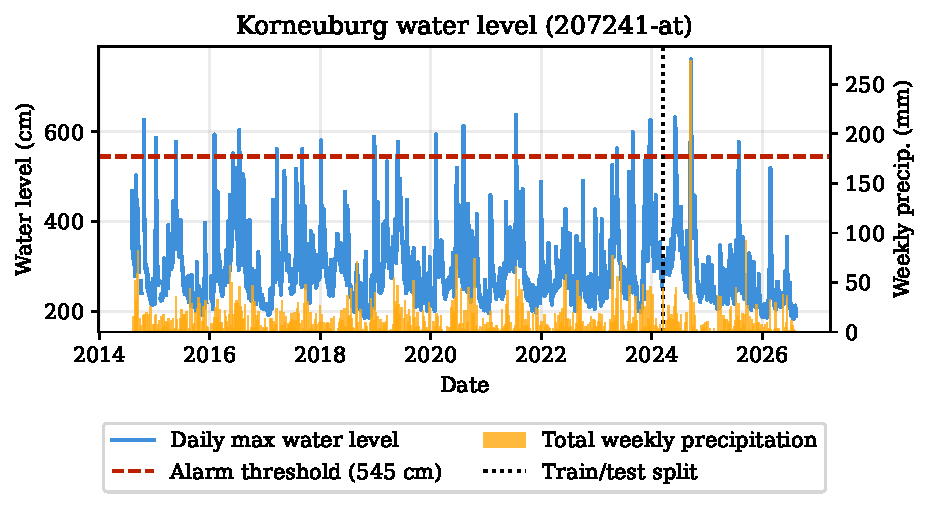
\includegraphics[width=\textwidth]{figures/target_water_level_history.pdf}
  \caption{Daily maximum water level at station 207241-at (in Korneuburg) over the full available period with weekly precipitation totals and the train/test split.}\label{fig:target-water-level-history}
\end{figure}

\autoref{fig:target-water-level-distribution} shows the distribution of observed hourly water levels at the target station. The distribution is right-skewed, with a long tail towards higher water levels. The first quartile is at 229 cm, the median is at 262 cm, and the third quartile is at 310 cm. The alarm threshold of 545 cm is far above the third quartile, values above the threshold are rare, with only 760 observations (0.75\% of the total) exceeding the threshold. 
% \autoref{fig:target-water-level-distribution}: Number of observations above alarm threshold: 760 (0.75%) Quartiles: Q1=229.00, Q2=262.00, Q3=310.00
\begin{figure}[htbp]
  \centering
  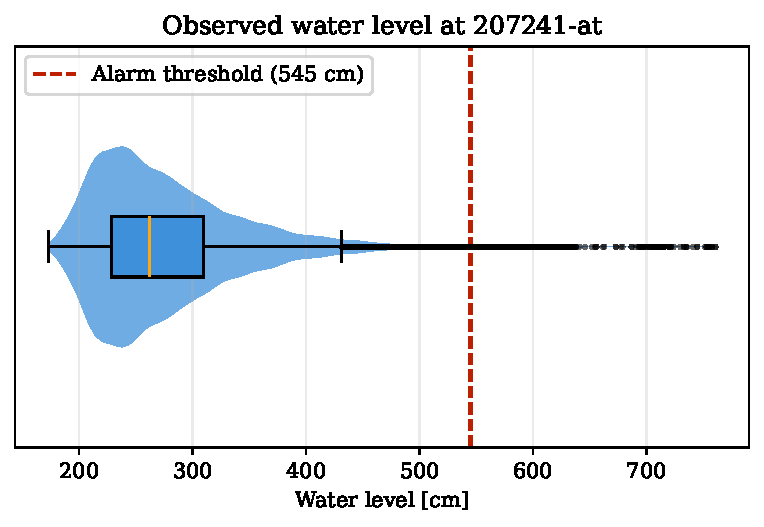
\includegraphics[width=\textwidth]{figures/target_water_level_distribution.pdf}
  \caption{Distribution of observed hourly water levels at the target station.}\label{fig:target-water-level-distribution}
\end{figure}


\autoref{fig:station-monthly-data-completeness} outlines the monthly availability of water level measurements across all eligible stations, as well as the proportion of rows that are eligible for use in the model. 207340-at, 207027-at and 207019-at have a later start date than the other stations, they are missing all measurements before mid 2015. Overall the availability of water level measurements is quite good, with the lowest availability being about 89\%. There are also some patterns in the missingness of the data. For example late 2015 and early 2016 there are some months with lower availability, of the same three stations. The reason could be that there is was an issue at the measurement station operator's side, or that FloodAlert was not able to fetch the data for some other reason (e.g. outage of their system). The proportion of rows that are eligible for use in the model training is comparatively low, since it requires that all features are available. This is due to several factors, the first one being that the the target must not be null for the entire 24 hour forecast horizon. A single null value in the target will make the many rows ineligible. Furthermore, all features must not be null for for the row to be eligible. Nevertheless the total number of eligible rows is still quite high with about 70,000 rows.
\begin{figure}[htbp]
  \centering
  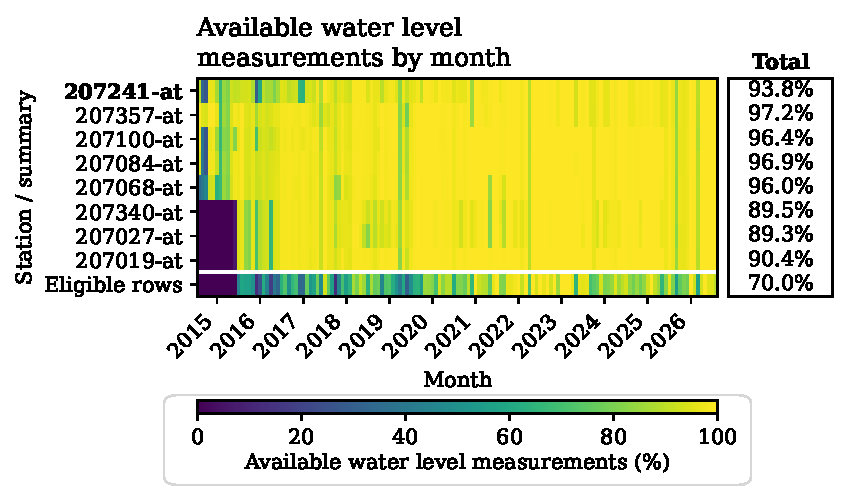
\includegraphics[width=\textwidth]{figures/station_monthly_data_completeness.pdf}
  \caption{Monthly available water level measurements and eligible rows for upstream stations (interpolated measurements count as missing).}\label{fig:station-monthly-data-completeness}
\end{figure}


The Pearson cross-correlation between upstream stations and the target station for lags of 0--72 hours is shown in \autoref{fig:upstream-cross-correlation-heatmap}. The plot indicates how many hours later the target station's measurements are most strongly correlated with the upstream stations' measurements. A lag of e.g. 2 hours before Korneuburg means that the upstream station's measurement at time $t$ is compared with Korneuburg's measurement two hours later ($t+2$). The circles in the plot mark the highest correlation for each station, which provides an indication of the propagation delay of water level changes. The stations are sorted by the distance to the target station, with the closest station at the top. With increasing lags the correlation decreases with the lowest correlation at 72 hours being between 0.66 and 0.75 All stations have their highest correlation with Kroneuburg at a lag of 2--7 hours. Except 207084-at, all stations also have a very high correlation of 0.95 or higher. It is not clear why the highest correlation for 207084-at is only 0.89. The lag associated with the maximum correlation generally increases for stations farther upstream. Station 207084-at is an exception to this pattern, reaching its maximum correlation at a lag of 7 hours, while the following two stations, both peak at a lag of 6 hours.
\begin{figure}[htbp]
  \centering
  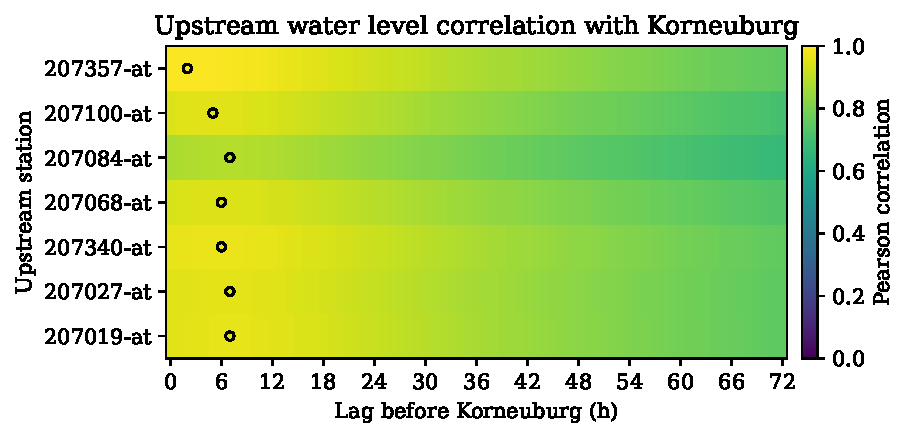
\includegraphics[width=\textwidth]{figures/upstream_cross_correlation_heatmap.pdf}
  \caption{Pearson cross-correlation between upstream stations and Korneuburg for lags of 0-72 hours. Positive lag means the upstream measurement leads Korneuburg; circles mark each station's peak.}\label{fig:upstream-cross-correlation-heatmap}
\end{figure}

The heatmap in \autoref{fig:weather-future-change-spearman} shows the Spearman correlation between precipitation sums, temperature means and subsequent water level changes at the target station. There is virtually no linear correlation between the temperature and future water level changes, with the highest correlation being 0.04 showing no monotonic relationship between the mean temperature and the future water level changes. The precipitation sums show a larger weak correlation with future water level changes, with the highest correlation being 0.26. Increased precipitation over the previous 6 and 24 hours is associated with the strongest subsequent water level changes  12 or 24 hours later. The correlation pattern suggests a delayed association between recent precipitation and water level changes. The weak negative correlation for the 72-hour precipitation sum at the 48-hour horizon may indicate that the water level has already risen due to earlier rainfall and is beginning to fall again. Additionally, the long 72-hour window makes it difficult to determine when exactly the precipitation occurred.
\begin{figure}[htbp]
  \centering
  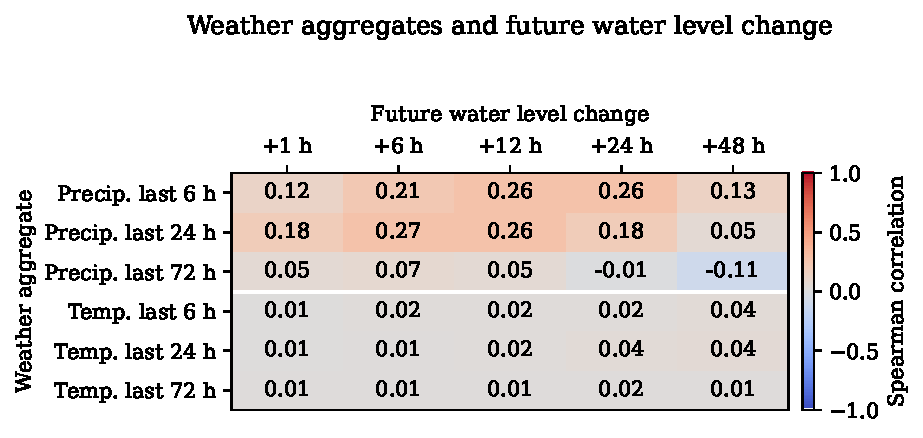
\includegraphics[width=\textwidth]{figures/weather_future_change_spearman.pdf}
  \caption{Spearman correlations between precipitation sums / temperature means and future water level changes at the target station.}\label{fig:weather-future-change-spearman}
\end{figure}



% TODO TAlk about hyperparameter spaces searched
\section{Model Performance}
Compare all model performances and select best model
\section{Feature Effects}
Investigate feature importance and effects on the model performance

\section{Forecast Analysis}
In depth analysis of the forecast performance (e.g.) e.g. performance over lead time, ... for the best/chosen model

\section{Deployment}
Deployment (Docker + FastAPI)

\chapter{Discussion}


\section{Main findings}


\section{Comparison with previous work}


\section{Implications}


\section{Limitations}

\section{Further Research}

% Document your AI tools here. They will automatically be added to a table.
% \aitoolentry{DeepL Translate}{Translation of an article in English}{Source (XXX), Chapter X on page X-X}
% \aitoolentry{Chat GPT 4.0}{Grammar and Spelling}{"Please list issues with spelling and grammar in the following text: ...", Entire document}
\aitoolentry{ChatGPT ($5.6$ Sol, Terra and Luna)}{Coding Assistance}{Code review, code completion and code generation}
\aitoolentry{Claude (Sonnet 5, Opus 5)}{Coding Assistance}{Code review, code completion and code generation}
\aitoolentry{ChatGPT ($5.6$ Sol, Terra and Luna)}{Grammar and Spelling}{Grammar, spelling and helping with wording \& translation throughout the entire document}
\aitoolentry{Claude (Sonnet 5, Opus 5)}{Grammar and Spelling}{Grammar, spelling and helping with wording \& translation throughout the entire document}

%
% The lists begin here.
%
\clearpage
\printbibliography
\clearpage

% List of figures
\listoffigures
\clearpage

% List of tables
\listoftables
\clearpage

% List of AI tools used
\listaitools
\clearpage

\phantomsection
\addcontentsline{toc}{chapter}{\listacroname}
\chapter*{\listacroname}
\begin{acronym}[XXXXX]
    \acro{RQ}{Research Question}
    \acro{INCA}{Integrated Nowcasting through Comprehensive Analysis}
    \acro{EDA}{Exploratory Data Analysis}
    \acro{MIMO}{Multiple-Input Multiple-Output}
    \acro{CV}{Cross-Validation}
    \acro{RMSE}{Root Mean Squared Error}
    \acro{MAE}{Mean Absolute Error}
    \acro{ME}{Mean Error}
    \acro{MLP}{Multilayer Perceptron}
    \acro{RNN}{Recurrent Neural Network}
    \acro{GRU}{Gated Recurrent Unit}
    \acro{LSTM}{Long Short-Term Memory}
\end{acronym}

%
% The appendix begins here.
%
\clearpage
\appendix
\chapter{Appendix Forecast Analysis}

\label{sec:appendix-forecast-analysis}
% test
\begin{figure}[htbp]
  \centering
  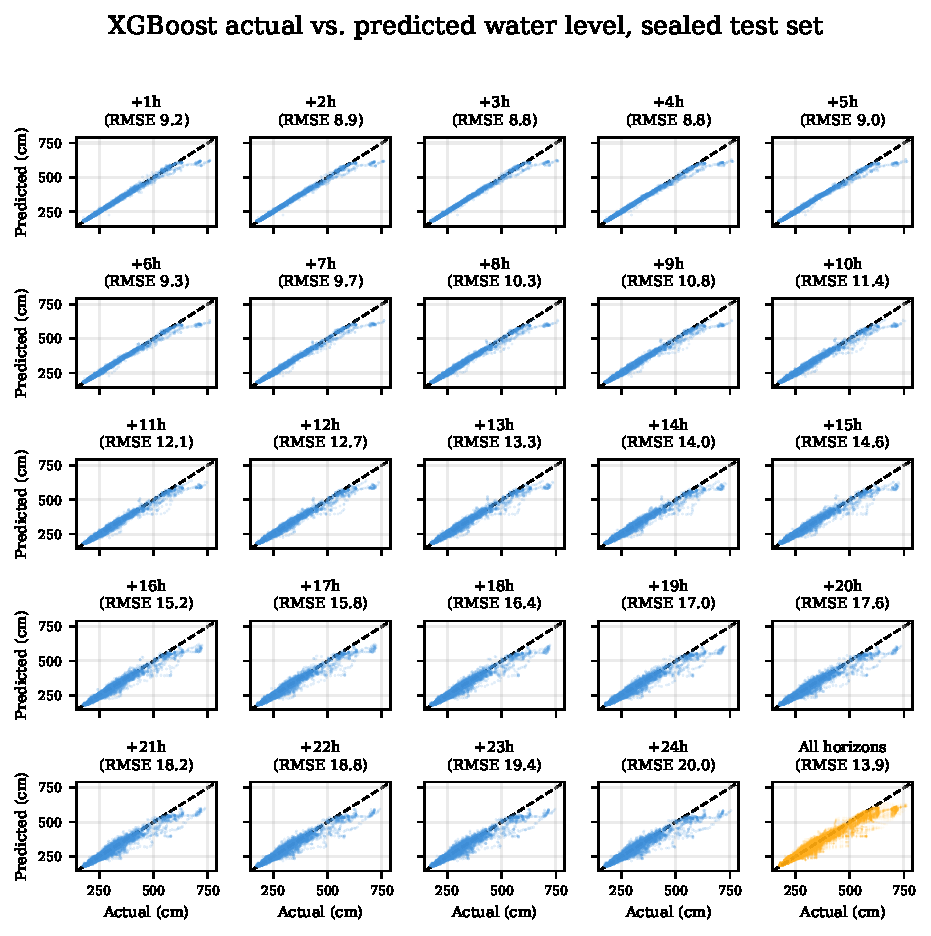
\includegraphics[width=\textwidth]{figures/xgboost_actual_vs_predicted_by_horizon.pdf}
  \caption{Actual versus predicted water level on the sealed test set for the XGBoost model, shown separately for each of the 24 forecast horizons and pooled across all horizons (bottom right). The dashed diagonal marks perfect agreement.}\label{fig:xgboost-actual-vs-predicted-by-horizon}
\end{figure}

\section{Hyperparameter Search Spaces}
\label{sec:hyperparameter-search-spaces}
\begin{table}[htbp]
  \centering
  \begin{tabularx}{\textwidth}{@{}lXr@{}}
\toprule
\textbf{Subset} & \textbf{Description} & \textbf{Features} \\
\midrule
Full & All predictor columns for every station: hydrology, quality/time, and weather. & 73 \\
\addlinespace
All-station hydrology, quality \& time & Hydrology, data-quality, and time features for every station; excludes weather. & 49 \\
\addlinespace
Raw, all stations & Raw (unengineered) water level and weather predictors for every station. & 32 \\
\addlinespace
Target-station full & All predictor columns for the target station only: hydrology, quality/time, and weather. & 45 \\
\addlinespace
Target-station hydrology, quality \& time & Hydrology, data-quality, and time features for the target station only; excludes weather. & 35 \\
\addlinespace
Current water levels, all stations & Current water level reading only, for every station. & 8 \\
\bottomrule
\end{tabularx}

  \caption{Definition of the six input feature subsets.}\label{tab:feature-subset-definitions}
\end{table}
\begin{table}[htbp]
  \centering
  \begin{tabularx}{\textwidth}{@{}lX@{}}
\toprule
\textbf{Hyperparameter} & \textbf{Search space} \\
\midrule
feature subset & \{Full; All-station hydrology, quality, and time; Raw all stations; Target station full; Target-station hydrology, quality, and time; Current water levels from all stations\} \\
\addlinespace
alpha & \{0.01, 0.1, 1.0, 10.0, 100.0\} \\
\addlinespace
log1p target & \{False, True\} \\
\bottomrule
\end{tabularx}

  \caption{Ridge hyperparameter search space. Exhaustive grid: 5 alpha values x 2 log1p settings x 6 feature subsets.}\label{tab:hyperparameter-search-space-ridge}
\end{table}

\begin{table}[htbp]
  \centering
  \begin{tabularx}{\textwidth}{@{}lX@{}}
\toprule
\textbf{Hyperparameter} & \textbf{Search space} \\
\midrule
feature subset & \{Full; All-station hydrology, quality, and time; Raw all stations; Target station full; Target-station hydrology, quality, and time; Current water levels from all stations\} \\
\addlinespace
hidden\_layer\_sizes & \{32, 64, 128, 256, 64x32, 128x64\} \\
\addlinespace
alpha & LogUniform(1e-05, 1) \\
\bottomrule
\end{tabularx}

  \caption{MLP hyperparameter search space. Random search: 16 candidates per feature subset (6 subsets).}\label{tab:hyperparameter-search-space-mlp}
\end{table}

\begin{table}[htbp]
  \centering
  \begin{tabularx}{\textwidth}{@{}lX@{}}
\toprule
\textbf{Hyperparameter} & \textbf{Search space} \\
\midrule
feature subset & \{Full; All-station hydrology, quality, and time; Raw all stations; Target station full; Target-station hydrology, quality, and time; Current water levels from all stations\} \\
\addlinespace
max\_depth & Uniform integer in [3, 7] \\
\addlinespace
learning\_rate & LogUniform(0.01, 0.3) \\
\addlinespace
n\_estimators & Uniform integer in [100, 500] \\
\addlinespace
subsample & Uniform(0.6, 1) \\
\addlinespace
colsample\_bytree & Uniform(0.6, 1) \\
\addlinespace
reg\_lambda & LogUniform(0.1, 10) \\
\bottomrule
\end{tabularx}

  \caption{XGBoost hyperparameter search space. Random search: 32 candidates per feature subset (6 subsets).}\label{tab:hyperparameter-search-space-xgboost}
\end{table}

\begin{table}[htbp]
  \centering
  \input{tables/hyperparameter_search_space_random_forest.tex}
  \caption{Random Forest hyperparameter search space. Random search: 12 candidates per feature subset (6 subsets).}\label{tab:hyperparameter-search-space-random-forest}
\end{table}

\begin{table}[htbp]
  \centering
  \begin{tabularx}{\textwidth}{@{}lX@{}}
\toprule
\textbf{Hyperparameter} & \textbf{Search space} \\
\midrule
feature subset & \{Full; All-station hydrology, quality, and time; Raw all stations; Target station full; Target-station hydrology, quality, and time; Current water levels from all stations\} \\
\addlinespace
n\_estimators & Uniform integer in [200, 800] \\
\addlinespace
max\_depth & \{8, 16, 32, None\} \\
\addlinespace
min\_samples\_leaf & Uniform integer in [1, 8] \\
\addlinespace
max\_features & \{sqrt, 0.5, 1.0\} \\
\bottomrule
\end{tabularx}

  \caption{Extra Trees hyperparameter search space. Random search: 24 candidates per feature subset (6 subsets).}\label{tab:hyperparameter-search-space-extra-trees}
\end{table}

\begin{table}[htbp]
  \centering
  \begin{tabularx}{\textwidth}{@{}lX@{}}
\toprule
\textbf{Hyperparameter} & \textbf{Search space} \\
\midrule
feature subset & \{Raw all stations\} \\
\addlinespace
cell\_type & \{gru, lstm\} \\
\addlinespace
sequence\_length & \{24\} \\
\addlinespace
hidden\_size & Uniform integer in [16, 128] \\
\addlinespace
num\_layers & Uniform integer in [1, 3] \\
\bottomrule
\end{tabularx}

  \caption{RNN hyperparameter search space. Random search: 16 candidates, raw all-stations input only.}\label{tab:hyperparameter-search-space-rnn}
\end{table}
\newpage

\section{Feature Subset Performance Comparison}
\label{sec:feature-subset-performance-comparison}
\begin{table}[htbp]
  \centering
  \begin{tabularx}{\textwidth}{@{}Xrr@{}}
\toprule
\textbf{Comparison} & \textbf{CV RMSE} & \textbf{Change in RMSE} \\
\midrule
Target station only (Target-station hydrology, quality \& time) & $16.18$ & reference \\
\addlinespace
+ neighboring stations (All-station hydrology, quality \& time) & $14.44$ & $-10.7\%$ \\
\addlinespace
+ weather (Target-station full) & $15.49$ & $-4.3\%$ \\
\addlinespace
+ neighboring stations + weather (Full) & $13.32$ & $-17.6\%$ \\
\bottomrule
\end{tabularx}

  \caption{\ac{CV} \ac{RMSE} for Ridge for different feature-subset configurations. Changes are relative to the target station only row.}\label{tab:feature-subset-performance-comparison-ridge}
\end{table}

\begin{table}[htbp]
  \centering
  \begin{tabularx}{\textwidth}{@{}Xrr@{}}
\toprule
\textbf{Comparison} & \textbf{CV RMSE} & \textbf{Change in RMSE} \\
\midrule
Target station only (Target-station hydrology, quality \& time) & $16.44$ & $\text{reference}$ \\
\addlinespace
+ neighboring stations (All-station hydrology, quality \& time) & $14.42$ & $-12.29\%$ \\
\addlinespace
+ weather (Target-station full) & $15.92$ & $-3.18\%$ \\
\addlinespace
+ neighboring stations + weather (Full) & $12.64$ & $-23.14\%$ \\
\bottomrule
\end{tabularx}

  \caption{\ac{CV} \ac{RMSE} for MLP for different feature-subset configurations. Changes are relative to the target station only row.}\label{tab:feature-subset-performance-comparison-mlp}
\end{table}

\begin{table}[htbp]
  \centering
  \begin{tabularx}{\textwidth}{@{}Xrr@{}}
\toprule
\textbf{Comparison} & \textbf{CV RMSE} & \textbf{Change in RMSE} \\
\midrule
Target station only (Target-station hydrology, quality \& time) & $16.93$ & reference \\
\addlinespace
+ neighboring stations (All-station hydrology, quality \& time) & $14.91$ & $-11.9\%$ \\
\addlinespace
+ weather (Target-station full) & $16.60$ & $-1.9\%$ \\
\addlinespace
+ neighboring stations + weather (Full) & $13.45$ & $-20.6\%$ \\
\bottomrule
\end{tabularx}

  \caption{\ac{CV} \ac{RMSE} for Extra Trees for different feature-subset configurations. Changes are relative to the target station only row.}\label{tab:feature-subset-performance-comparison-extra-trees}
\end{table}

% \todo{Change this to the actual appendix}
\clearpage
\chapter{Appendix B}
\end{document}
